\documentclass[a4paper,10pt]{report}
\usepackage[utf8x]{inputenc}
\usepackage{amsmath}
\usepackage{amsfonts}
\usepackage{natbib}
\usepackage{graphicx} % figuras
\usepackage[export]{adjustbox} % loads also graphicx
\usepackage{float}
\usepackage{amssymb}

% Title Page
\title{Two-phase flow}
\author{}


\begin{document}
% \chapter{Two-phase flow}
% \section{Two-phase flow.}
% When simulating two phases within a porous medium, we often consider them as separated phases, i.e.,
% they are inmiscible and there is no mass transfer between the phases. 
% The contact between phases is known as the interface between two reservoir fluids phases.\\ 
% While modeling two phases, we 
% usually consider one of the fluids as the wetting phase ($w$) that wets the porous medium more than the other.
% The other phase is consider as non-wetting phase ($n$). In the case of a water-oil system, water is often 
% the wetting phase. \\
% For a reservoir, the density of each phase varies, the gas is less dense than the oil and water. 
% Therefore, the gas is found on top of the reservoir. For the oil-water system, water's density is larger 
% than oil's, then water is found on the bottom of the reservoir.\\
% The saturation of a phase $S_{\alpha},$ is the fraction of void space filled with that phase in a porous 
% medium.
% If there are two phases present in the porous medium, these fluids fill completely the empty space, which is
% expressed by the following relation.
% \begin{equation}\label{eq:satrel}
%  S_n+S_w=1
% \end{equation}
% 
% The surface tension and the curvature of the interface between the fluids causes a difference in pressure
% between the two phases. 
% The pressure in the wetting fluid is less than in the nonwetting fluid. 
% This difference in pressures is known as the capillary pressure, $p_c$, and it's function of saturation:
% \begin{equation}\label{eq:cappress}
%  p_c(S_w)=p_n-p_w.
% \end{equation}
% As mentioned before, the pressure in the non-wetting fluid is higher than the pressure in the wetting fluid, therefore the 
% capillary pressure is always positive. 
% The relation between the capillary pressure and saturation is obtained as an empirical model based on experiments. 
% However, each core sample will have different capillary curve due to the difference in pore-size distributions,
% porosity and permeability.
% To normalize the measured data, it's common to use a so-called Leverett J-function, which takes the following form:
% 
% \begin{equation}
%  J(S_w)=\frac{P_c}{\sigma cos \theta}\sqrt{\frac{K}{\phi}},
% \end{equation}
% where $\sigma$ is the surface tension and $\theta$ the contact angle measured in the laboratory for an specific rock and fluid system.\\
% A model that relates the capillary pressure and water saturation in a partially saturated media (water and air media) is:
% 
% \begin{equation*}
% \hat{S}_w=
% \begin{cases}
% (p_c/p_e)^{-n_b} & \text{ if } p_c>p_e\\
% 1& p_c \leq p_e
% \end{cases}
% \end{equation*}
% where $p_e$ is the entry pressure of air, and $n_b$ is related to the pore-size distribution. This model was proposed by Brooks and Corey.
% Another model was proposed by Genuchten:
% \begin{equation}
%  \hat{S}_w=\left( 1+(\beta_gp_c)^n_g)^{-m_g}\right),
% \end{equation}
% where $\beta_g$ is related to the average size of pores and $n_g$ and $m_g$ are related to the pore size distribution. \\
% \emph{Relative permeability}\\
% When more than one phase is present in the pore space, each phase $\alpha$ will experience an effective permeability $K_{\alpha}^ e$that is less than the absolute permeability $K$. Due to interfacial tensions, the sum of all the phase permeabilities is less than one.
% $$\sum_{\alpha}K_{\alpha}^e<K.$$
% The relative permeability for an isotropic medium is defined as:
% $$k_{r\alpha}=K_{\alpha}^e/K.$$
% The relative permeabilities will generally be functions of saturation, generally nonlinear.
% It is common to use analytic relationships to represent relative permeabilities. These are usually stated using normalized or effective saturations $\hat{S}_w.$ The simplest model possible is called the Corey model:
% \begin{equation}\label{eq:Corey}
% \begin{aligned}
% k_{rw}=(\hat{S}_w)^{n_w}k_w^0,\\
% k_{ro}=(1-\hat{S}_w)^{n_n}k_o^0.\\
% \end{aligned}
% \end{equation}
% where $n_w>1$, $n_o>1$ and $k_{\alpha}^0$ are fitting parameters.\\
% The Brooks-Corey functions are also used. 
% \begin{equation*}
% \begin{aligned}
% k_{rw}=(\hat{S}_w)^{n_1+n_2n_3},\\
% k_{ro}=(1-\hat{S}_w)^{n_1}[1-(\hat{S}_w)^{n_2}]^{n_3}.\\
% \end{aligned}
% \end{equation*}
% where, $n_1 = 2$, $n_2 = 1 + 2/n_b$ and $n4 = 1$ for the Brooks–Corey–Burdine model and $n_1 = \eta$, $n_2 = 1 + 1/n_b$ and $n3 = 2$ for the Brooks–Corey–Mualem model. For the van Genuchten capillary functions $m_g = 1 − 1/n_g$) we have:
% \begin{equation*}
% \begin{aligned}
% k_{rw}=\hat{S}_w^2[1-(1-\hat{S}_w^{1/m_g})^{m_g}],\\
% k_{ro}=(1-\hat{S}_w)^2[1-(\hat{S}_w^{1/m_g})]^{m_g},\\
% \end{aligned}
% \end{equation*}
% which is called the Genuchten-Burdine model.\\
% % If we have an oil reservoir  with volume $V$ and porosity $\phi$ the oil volume
% % in reservoir (OIP-oil in place) is given by:
% % $$OIP=V\phi (1-S_{wc})$$
% % Where $S_{wc}$ is the irreducible water saturation, the water present in the oil and gas zones of the
% % reservoir, also known as connate water. 
% % If the oil is generated in deep rock, when it moves to an upper 
% % zone filled with water, it cannot displace all the water. This water remain as connate water, normally 
% % between 10 and 15 \%.
% As in the single-phase case, the governing equations for two-phase flow in a porous medium are the mass 
% conservation and Darcy's law. 
% The mass balance equations for each phase $\alpha$ are given by:
% \begin{equation*}
%  \frac{\partial(\phi \rho_{\alpha}S_{\alpha})}{\partial t}+\nabla \cdot ( \rho_{\alpha} \mathbf{v}_{\alpha})=\rho_{\alpha} q_{\alpha},
% \end{equation*}
% 
% Darcy's law is:
% \begin{equation*}
% \mathbf{v}_{\alpha}=-\frac{k_{r\alpha}}{\mu_{\alpha}} {K}(\nabla p_{\alpha}-\rho_{\alpha} g \nabla z).
% \end{equation*}
% To simplify notation, the phase mobilities ($\lambda_{\alpha}=Kk_{r\alpha}/\mu_{\alpha}$) or relative phase mobilities ($\lambda_{\alpha}=\lambda_{\alpha}K$) are used. 
% Using the discrete derivative operators and backward discretization of temporal derivatives, the resulting system of discrete equations is:
% \begin{equation*}
%  \frac{(\phi \mathbf{\rho}_{\alpha}\mathbf{S}_{\alpha})^{n+1}-(\phi \mathbf{\rho}_{\alpha}\mathbf{S}_{\alpha})^{n}}{\Delta t^n}+div  ( \mathbf{\rho}_{\alpha} \mathbf{v}_{\alpha})^{n+1}= \mathbf{q}_{\alpha}^{n+1},
% \end{equation*}
% 
% \begin{equation*}
% \mathbf{v}_{\alpha}^{n+1}=-\frac{\mathbf{k}_{r\alpha}}{\mathbf{\mu}_{\alpha}} \mathbf{K}[grad( \mathbf{p}_{\alpha}^{n+1})-g\mathbf{\rho}_{\alpha}^{n+1}  grad(\mathbf{z})].
% \end{equation*}
% \emph{Immiscible two-phase flow}\\
% For the case of immiscible fluids, the flow equations are:
% \begin{equation}\label{we}
%  \frac{\partial(\phi \rho_{w}S_{w})}{\partial t}+\nabla \cdot ( \rho_{w} \mathbf{v}_{w})=\rho_{w} q_{w},
% \end{equation}
% \begin{equation}\label{ne}
%  \frac{\partial(\phi \rho_{n}S_{.})}{\partial t}+\nabla \cdot ( \rho_{n} \mathbf{v}_{n})=\rho_{n} q_{n}.
% \end{equation}
% \emph{Pressure formulation}\\
% We can choose the pressures as the primary unknowns, then the saturations are expressed as functions of pressure. 
% Assuming the capillary pressure has a unique inverse function $\hat{S}_w=P_c^{-1}(p_c)$, then we have:
% $$S_w=\hat{S}_w(p_n-p_w)\qquad S_n=1-\hat{S}_w(p_n-p_w), $$
% then equations \eqref{we} and \eqref{ne} can be written as:
% \begin{equation}
%  \frac{\partial(\phi \rho_{w}\hat{S}_{w})}{\partial t}+\nabla \cdot ( \rho_{w} \frac{{K}k_{rw}(\hat{S}_w)}{\mu_w}(\nabla p_w-\rho_w g \nabla z))=\rho_{w} q_{w},
% \end{equation}
% \begin{equation}
%  \frac{\partial(\phi \rho_{n}(1-\hat{S}_{w}))}{\partial t}+\nabla \cdot ( \rho_{n} \frac{{K}k_{rn}(\hat{S}_w)}{\mu_n}(\nabla p_n-\rho_n g \nabla z))=\rho_{n} q_{n}.
% \end{equation}
% Previous system is highly coupled and strongly nonlinear. \\
% \emph{Fractional flow formulation}\\
% Part of the non linearity of previous formulation can be eliminated if the system is expressed in terms of one phase pressure and one phase saturation. A common choice is to use $p_n$ and $S_w$ which gives the following system
% \begin{equation}
%  \frac{\partial(\phi \rho_{w}{S}_{w})}{\partial t}+\nabla \cdot ( \rho_{w} \frac{{K}k_{rw}}{\mu_w}(\nabla p_n-\nabla P_c(S_w)-\rho_w g \nabla z))=\rho_{w} q_{w},
% \end{equation}
% \begin{equation}
%  \frac{\partial(\phi \rho_{n}(1-{S}_{w}))}{\partial t}+\nabla \cdot ( \rho_{n} \frac{{K}k_{rn}}{\mu_n}(\nabla p_n-\rho_n g \nabla z))=\rho_{n} q_{n}.
% \end{equation}
% 
% \emph{Incompressible flow}\\
% For incompressible flow, only the Saturation $S$ is a function of time and the fluid densities $\rho_{\alpha}$ are constant. Therefore, the mass-balance equations are:
% \begin{equation}
%  \phi\frac{\partial( {S}_{\alpha})}{\partial t}+\nabla \cdot ( \mathbf{v}_{\alpha})= q_{\alpha}.
% \end{equation}
% The total Darcy velocity is defined as the sum of the velocity in the wetting and non wetting phases, it can be expressed in terms of the non-wetting phase as:
% \begin{align*}
% \mathbf{v}=\mathbf{v}_w+\mathbf{v}_n=-\lambda_{n}\nabla p_n-\lambda_{w}\nabla p_w+(\lambda_n \rho_n+\lambda_w\rho_w)g\nabla z\\
% =-(\lambda_n+\lambda_w)\nabla p_n+\lambda_w\nabla p_c+(\lambda_n \rho_n+\lambda_w\rho_w)g\nabla z
% \end{align*}
% if we add the two continuity equations and use the relationship $S_n+S_w=1$ we have:
% \begin{equation*}
%  \phi\frac{\partial( {S}_{w}+S_n)}{\partial t}+\nabla \cdot ( \mathbf{v}_{w}+\mathbf{v}_n)= q_{n}+q_w.
% \end{equation*}
% Using $\lambda=\lambda_n+\lambda_w=\lambda K$ as the total mobility and $q=q_n+q_w$ as the total source, for the total Darcy velocity we have:
% \begin{align*}
% -\nabla \cdot (\lambda K\nabla p_n)=q-\nabla[\lambda_w\nabla p_c+(\lambda_n\rho_n+\lambda_w\rho_w)g\nabla z].
% \end{align*}
% Multiplying each phase velocity by the relative mobility of the other phase and subtracting the result we obtain:
% \begin{align*}
% \lambda_n\mathbf{v}_w-\lambda_w\mathbf{v}_n&=\lambda\mathbf{v}_w-\lambda_w\mathbf{v}\\
% &=\lambda_w\lambda_n K[\nabla p_c+(\rho_w-\rho_n)g\nabla z].
% \end{align*}
% Therefore, for $\mathbf{v}_w$ we have
% \begin{align*}
% \mathbf{v}_w=\frac{\lambda_w}{\lambda}\mathbf{v}+\frac{\lambda_w\lambda_n}{\lambda} K[\nabla p_c+(\rho_w-\rho_n)g\nabla z].
% \end{align*}
% Using the velocity computed above, for the wetting phase we have:
% \begin{equation}\label{eq:sat}
%  \phi\frac{\partial( {S}_{w})}{\partial t}+\nabla \cdot [f_w( \mathbf{v}+\lambda_n\Delta  \rho g\nabla z)]= q_w-\nabla \cdot(f_w\lambda_np_c\nabla S_w).
% \end{equation}
% with $\Delta \rho= \rho_w-\rho_n$ and the fractional flow function $f_w$:
% $$f_w=\frac{\lambda_{w}}{\lambda_n+\lambda_w},$$
% is the fraction of the total flow that consists of the wetting fluid, and
% \begin{align*}
% \mathbf{v}=-\lambda(\nabla p_n-f_w\nabla p_w-(f_n \rho_n+f_w\rho_w)g\nabla z)\\
% \end{align*}
% 
% The coupling between the elliptic pressure equation and the parabolic saturation equation is much weaker than the coupling between the two continuity
% equations in the two-pressure formulation. In the pressure equation,
% the coupling to saturation appears explicitly in the effective mobility that makes up the variable coefficient in the Poisson problem and on the
% right-hand side through the phase mobilities and the derivative of the capillary function. In Equation \eqref{eq:sat}, the saturation is only indirectly
% coupled to the pressure through the total Darcy velocity. \\
% The system of PDEs can then be reformulated so that
% it consists of an elliptic equation for fluid pressure and one or more transport equations. These transport equations are generally parabolic, but have a
% strong hyperbolic character. Since the pressure and saturations equations have very different mathematical characteristics, it is natural
% to solve them in consecutive substeps. Sequential solution procedures and in-
% compressible flow models are popular in academia and for research purposes,
% but are less used in industry. To the extent simulations are used for practical reservoir engineering, they are mainly based on compressible equations
% and solution procedures in which flow and transport are solved as a coupled
% system. Such approaches are very robust and particularly useful for problems
% with large variations in time constants or strong coupling between different
% types of flow mechanisms. \\\\\\
% \emph{\textbf{Sequential solution procedures}}\\
% The two-phase, incompressible model will be solved using the fractional-flow formulation. This fractional flow model consists of an elliptic
% pressure equation
% \begin{equation}\label{eq:wdarcy}
%  \nabla \cdot \mathbf{v}=q, \qquad \mathbf{v}=-\lambda(\nabla p_n-f_w\nabla p_c-(f_n \rho_n+f_w\rho_w)g\nabla z)\\
% \end{equation}
% and a parabolic transport equation \eqref{eq:sat}
% \begin{equation}\label{eq:wsat}
%  \phi\frac{\partial( {S}_{w})}{\partial t}+\nabla \cdot [f_w( \mathbf{v}+\lambda_n(\Delta  \rho g\nabla z)+\nabla P_c)]= q_w.
% \end{equation}
% Where the capillary pressure $p_c = p_w −p_n$ is assumed to be a known function $P_c$ of the wetting saturation $S_w$. The transport equation becomes hyperbolic whenever $P_c$ is zero.\\
% In the standard sequential solution procedure, the system above, is
% evolved in time using a set of discrete time steps $\Delta t_i$ . We assume that $p, \mathbf{v},$
% and $S_w$ are all known at time t and that we want to evolve the solution to time
% $t + \Delta t$.\\
% At the beginning of the time step, we first assume that the saturation
% $S_w$ is fixed. This means that the parameters $\lambda, f_w ,$ and $f_n$ are 
% functions of the spatial variable $\mathbf{x}$, and hence we can use this equation only to update the pressure $p_n$ and the Darcy velocity $\mathbf{v}$. Then, $\mathbf{v}$ and $p_n$ are held
% fixed while equation \ref{eq:wsat} is evolved a time step $\Delta t$ to define an updated saturation $S_w (\mathbf{x}, t + \Delta t)$. This saturation is then held fixed when we update $p_n$ and $\mathbf{v}$ in the next time step, and so on.
% Some authors refer to this solution procedure as an operator splitting
% method since the solution procedure effectively splits the overall solution operator of the flow model into two parts that are evolved in consecutive substeps.
% Likewise, some authors refer to the sequential solution procedure as IMPES,
% which is short-hand for implicit pressure, explicit saturation. Using the name
% IMPES is strictly speaking only correct if the saturation evolution is approximated by a single time step of an explicit transport solver.\\\\
% \emph{\textbf{Pressure solvers}}\\
% The pressure Equation \eqref{eq:wdarcy} for incompressible, multiphase flow is time dependent. This time dependence comes as the result of three factors:
% \begin{enumerate}
%  \item $K/\mu$ being replaced by the total mobility $\lambda(S_w )$, which depends on time through the saturation $S_w (\mathbf{x}, t + \Delta t)$,
%  \item the constant density $\rho$ being replaced by a saturation-dependent quantity $\rho_w f_w (S_w ) + \rho_nf_n (S_w )$, and
%  \item the source term $q$ being replaced by a saturation-dependent source term
% $q − \nabla \lambda_w (S_w )\nabla P_c (S_w )$.
% \end{enumerate}
% However, once $S_w$ is held fixed in time, all three quantities become functions of $\mathbf{x}$ only, and we hence end up again with an elliptic Poisson-type equation having the same spatial variation. \\
% \emph{Saturation solvers}\\
% The saturation equation depends on the time, using backward Euler discretization for the time derivative in Equation \ref{eq:wsat}, we have:
% \begin{equation}\label{eq:wsat1}
%  \phi\frac{( {S}_{w}^{n+1}-{S}_{w}^n)}{\Delta t}+\nabla \cdot [f_w({S}_{w})( \mathbf{v}+\lambda_n({S}_{w})(\Delta  \rho g\nabla z+\nabla P_c({S}_{w})))]= q_w,
% \end{equation}
% or
% \begin{equation*}\label{eq:wsat2}
%  {S}_{w}^{n+1}={S}_{w}^n-\frac{\Delta t}{\phi}\nabla \cdot [f_w({S}_{w})( \mathbf{v}+\lambda_n({S}_{w})(\Delta  \rho g\nabla z+\nabla P_c({S}_{w})))]+q_w,
% \end{equation*}
% which can be computed explicitly:
% \begin{equation*}\label{eq:wsat3}
%  {S}_{w}^{n+1}={S}_{w}^n-\mathcal{F}({S}_{w}^{n},{S}_{w}^{n}),
% \end{equation*}
% or implicitly:
% \begin{equation*}\label{eq:wsat4}
%  {S}_{w}^{n+1}={S}_{w}^n-\mathcal{F}({S}_{w}^{n+1},{S}_{w}^{n}).
% \end{equation*}
% If we use the implicit scheme, the system is nonlinear and depends on the saturation at time step $n$ and $n+1$.\\
% The discretization is implemented with the following residual form for each cell $\Omega_i$,
% \begin{equation}\label{eq:resS}
%  F_i (s, r) = s_i − r_i +\frac{\Delta t}{\phi_i|\Omega_i|}[H_i (s) − max(q_i, 0) − min(q_i , 0)f (S_i )],
% \end{equation}
% where $s$ and $r$ are cell-averaged quantities and subscript $i$ refers to
% the cell the average is evaluated in. The sum of the interface fluxes for cell $i$ 
% \begin{equation}
%  H_i (s) =\sum_k \frac{\lambda^u_w (s_i , s_k )}{\lambda^u_w (si , sk ) + \lambda^u_n (si , sk )}[v_{ik} + \lambda^u_n (s_i , s_k )(g_{ik} + P_{ik} )],
% \end{equation}
% is computed using the single-point upstream mobility-weighting, whereas the fractional flow function $f$ in the source term
% is evaluated from the cell average of $S$ in cell $\Omega_i$ . The explicit scheme is given
% as $S^{n+1} = S^n −F(S^n , S^n )$ and the implicit solution is obtained solving $F(S^{n+1} , S^{ n}) = 0$. 
% The residual equations \eqref{eq:resS} for all cells in vector form
% \begin{equation}
%  \mathbf{F} (\mathbf{s}) = \mathbf{s} − \mathbf{S} +\frac{\Delta t}{\phi_i|\Omega|}[\mathbf{H} (\mathbf{s}) − \mathbf{Q}^+ − \mathbf{Q}^-\mathbf{f} (\mathbf{S} )]=\mathbf{0}.
% \end{equation}
% Here, s is the unknown state at time $tf$ and S is the known state at the start
% of the time step. The nonlinear system can be solved with NR method, where, for the $(k+1)$-th iteration we have:
% 
% $$\mathbf{J}(\mathbf{S}^k)\delta\mathbf{S}^{k+1}=-\mathbf{F}(\mathbf{S}^k;\mathbf{S}^n),
% \qquad \mathbf{S}^{k+1}=\mathbf{S}^k+\delta \mathbf{S}^{k+1},$$
% where $\mathbf{J}(\mathbf{S}^k)=\frac{\partial \mathbf{F}(\mathbf{S}^k;\mathbf{S}^n)}{\partial \mathbf{S}^k}$ is the 
% Jacobian matrix, and $\delta \mathbf{S}^{k+1}$ is the NR update at iteration step $k+1$.\\
% Therefore, the linear system to solve is:\\
% \begin{equation}\label{eq:lsS}
% \mathbf{J}(\mathbf{pS}^k)\delta \mathbf{S}^{k+1}=\mathbf{b}(\mathbf{S}^k).
% \end{equation}
% with $\mathbf{b}(\mathbf{S}^k)$ being the function evaluated at iteration step $k$, $\mathbf{b}(\mathbf{S}^k)=-\mathbf{F}(\mathbf{S}^k;\mathbf{S}^n)$.\\
% 


\chapter*{Heterogeneous permeability 7 layers, no capillary pressure, X flux. 2 wells,bhp}
Layers with different permeability, 35 x 35 cells

\begin{table}[!ht]
\centering
\begin{tabular}{ |c|c|c|c|} 
\hline
Property&Water&Oil&Units\\
$\mu$&     1&    10 & $centi*poise$  \\  
$\rho$& 1000& 850& $kilogram/meter^3$\\
$k_r$&$(S_w)^2$&   $(1-S_w)^2$ &  \\
 \hline
\end{tabular}
\label{table:fluid}
\end{table} 


\begin{table}[!ht]\centering
\begin{minipage}{1\textwidth}
 \centering
\begin{tabular}{ ||c|c||c|c|c|c|c||} 
\hline
$\frac{\sigma_2}{\sigma_1}$&Total&Method  & ICCG&DICCG &Total&\% of total\\ 
                           & ICCG     &  & Snapshots& &ICCG& ICCG\\ 
                           \hline
$10^{0}$ &30965& DICCG$_{10}$&395&35878&36273&117\\ 
\hline  
$10^{0}$ &30965& DICCG$_{POD_{10}}$&395&2998&3393&11 \\ 
\hline  
$10^{0}$ &30965& DICCG$_{POD_{5}}$&395&4139&4534&15 \\ 
\hline  
$10^{1}$ &45283& DICCG$_{10}$&570&45991&46561&103\\ 
\hline  
$10^{1}$ &45283& DICCG$_{POD_{10}}$&570&3406&3976&9 \\ 
\hline  
$10^{1}$ &45283& DICCG$_{POD_{5}}$&570&4244&4814&11 \\ 
\hline  
$10^{2}$ &50111& DICCG$_{10}$&629&50236&50865&102\\ 
\hline  
$10^{2}$ &50111& DICCG$_{POD_{10}}$&629&3587&4216&8 \\ 
\hline  
$10^{2}$ &50111& DICCG$_{POD_{5}}$&629&4379&5008&10 \\ 
\hline 
$10^{3}$ &53476& DICCG$_{10}$&670&53615&54285&102\\ 
\hline  
$10^{3}$ &53476& DICCG$_{POD_{10}}$&670&3826&4496&8 \\ 
\hline  
$10^{3}$ &53476& DICCG$_{POD_{5}}$&670&4335&5005&9 \\ 
\hline 
\end{tabular} 
\caption{Comparison between the ICCC and DICCG methods of the average number of linear iterations for the second NR iteration for various contrast between permeability layers. }\label{table:litertot2} 
\end{minipage}  
\end{table}  




\begin{figure}[!h] \hspace{-1cm}
\begin{minipage}{.5\textwidth}
 \centering
\includegraphics[width=6cm,height=6cm,keepaspectratio]
{/home/wagm/cortes/Localdisk/Results/17_06/two_phases/30/2w/10-11_35perm_0cp0/def_0_pod_0/Permeability.jpg}
\caption{Rock perm.}
\label{fig:Convho}
\end{minipage}%  
\hspace{0.5cm}
\begin{minipage}{.5\textwidth}
 \centering
\includegraphics[width=6cm,height=6cm,keepaspectratio]
{/home/wagm/cortes/Localdisk/Results/17_06/two_phases/30/2w/10-11_35perm_0cp0/def_0_pod_0/bhp.jpg}
\caption{Bhp.}
\label{fig:Convho}
\end{minipage}
\end{figure}


\begin{figure}[!h] \hspace{-1cm}
\begin{minipage}{.5\textwidth}
 \centering
\includegraphics[width=6cm,height=6cm,keepaspectratio]
{/home/wagm/cortes/Localdisk/Results/17_06/two_phases/30/2w/10-11_35perm_0cp0/def_0_pod_0/Oil_rate.jpg}
\caption{Oil Rate.}
\label{fig:Convho}
\end{minipage}%  
\hspace{0.5cm}
\begin{minipage}{.5\textwidth}
 \centering
\includegraphics[width=6cm,height=6cm,keepaspectratio]
{/home/wagm/cortes/Localdisk/Results/17_06/two_phases/30/2w/10-11_35perm_0cp0/def_0_pod_0/Water_rate.jpg}
\caption{Water Rate.}
\label{fig:Convho}
\end{minipage}
\end{figure}



\begin{figure}[!h] \hspace{-1cm}
\begin{minipage}{.5\textwidth}
 \centering
\includegraphics[width=8cm,height=8cm,keepaspectratio]
{/home/wagm/cortes/Localdisk/Results/17_06/two_phases/30/2w/10-11_35perm_0cp0/def_0_pod_0/Water_saturation.jpg}
\caption{Water saturation.}
\label{fig:Convho}
\end{minipage}%  
\hspace{0.5cm}
\begin{minipage}{.5\textwidth}
 \centering
\includegraphics[width=8cm,height=8cm,keepaspectratio]
{/home/wagm/cortes/Localdisk/Results/17_06/two_phases/30/2w/10-11_35perm_0cp0/def_0_pod_0/Pressure.jpg}
\caption{Pressure.}
\label{fig:Convho}
\end{minipage}
\end{figure}


\newpage
\begin{figure}[!h] \hspace{-1cm}
\hspace{0.5cm}
\begin{minipage}{.5\textwidth}
 \centering
\includegraphics[width=6cm,height=6cm,keepaspectratio]
{/home/wagm/cortes/Localdisk/Results/17_06/two_phases/30/2w/10-11_35perm_3cp0/def_0_pod_0/bhp.jpg}
\caption{Bhp.}
\label{fig:Convho}
\end{minipage}%
\begin{minipage}{.5\textwidth}
 \centering
\includegraphics[width=6cm,height=6cm,keepaspectratio]
{/home/wagm/cortes/Localdisk/Results/17_06/two_phases/30/2w/10-11_35perm_1cp0/def_0_pod_0/Water_rate.jpg}
\caption{Water Rate (perm 10-1).}
\label{fig:Convho}
\end{minipage}  
\end{figure}


\begin{figure}[!h] \hspace{-1cm}
\begin{minipage}{.5\textwidth}
 \centering
\includegraphics[width=6cm,height=6cm,keepaspectratio]
{/home/wagm/cortes/Localdisk/Results/17_06/two_phases/30/2w/10-11_35perm_2cp0/def_0_pod_0/Water_rate.jpg}
\caption{Water Rate (perm 10-2).}
\end{minipage}%  
\hspace{0.5cm}
\begin{minipage}{.5\textwidth}
 \centering
\includegraphics[width=6cm,height=6cm,keepaspectratio]
{/home/wagm/cortes/Localdisk/Results/17_06/two_phases/30/2w/10-11_35perm_3cp0/def_0_pod_0/Water_rate.jpg}
\caption{Water Rate (perm 10 -3).}
\label{fig:Convho}
\end{minipage}
\end{figure}







\chapter*{Heterogeneous permeability 7 layers, no capillary pressure, X flux. 2 wells, rate}
Layers with different permeability, 35 x 35 cells

\begin{table}[!ht]
\centering
\begin{tabular}{ |c|c|c|c|} 
\hline
Property&Water&Oil&Units\\
$\mu$&     1&    10 & $centi*poise$  \\  
$\rho$& 1000& 850& $kilogram/meter^3$\\
$k_r$&$(S_w)^2$&   $(1-S_w)^2$ &  \\
 \hline
\end{tabular}
\label{table:fluid}
\end{table} 


\begin{table}[!ht]\centering
\begin{minipage}{1\textwidth}
 \centering
\begin{tabular}{ ||c|c||c|c|c|c|c||} 
\hline
$\frac{\sigma_2}{\sigma_1}$&Total&Method  & ICCG&DICCG &Total&\% of total\\ 
                           & ICCG     &  & Snapshots& &ICCG& ICCG\\ 
                           \hline
\hline 
$10^{0}$ &37089& DICCG$_{10}$&462&41878&42340&114\\ 
\hline  
$10^{0}$ &37089& DICCG$_{POD_{10}}$&462&31830&32292&87 \\ 
\hline  
$10^{0}$ &37089& DICCG$_{POD_{5}}$&462&32355&32817&88 \\ 
\hline 
\end{tabular} 
\caption{Comparison between the ICCC and DICCG methods of the average number of linear iterations for the second NR iteration for various contrast between permeability layers. }\label{table:litertot2} 
\end{minipage}  
\end{table}  




\begin{figure}[!h] \hspace{-1cm}
\begin{minipage}{.5\textwidth}
 \centering
\includegraphics[width=6cm,height=6cm,keepaspectratio]
{/home/wagm/cortes/Localdisk/Results/17_06/two_phases/30/2w/rate/10-11_35perm_1cp0/def_0_pod_0/Permeability.jpg}
\caption{Rock perm.}
\label{fig:Convho}
\end{minipage}%  
\hspace{0.5cm}
\begin{minipage}{.5\textwidth}
 \centering
\includegraphics[width=6cm,height=6cm,keepaspectratio]
{/home/wagm/cortes/Localdisk/Results/17_06/two_phases/30/2w/rate/10-11_35perm_0cp0/def_0_pod_0/bhp.jpg}
\caption{Bhp, homogeneous perm.}
\label{fig:Convho}
\end{minipage}
\end{figure}


\begin{figure}[!h] \hspace{-1cm}  
\hspace{0.5cm}
\begin{minipage}{.5\textwidth}
 \centering
\includegraphics[width=6cm,height=6cm,keepaspectratio]
{/home/wagm/cortes/Localdisk/Results/17_06/two_phases/30/2w/rate/10-11_35perm_0cp0/def_0_pod_0/Water_rate.jpg}
\caption{Water Rate.}
\label{fig:Convho}
\end{minipage}%
\begin{minipage}{.5\textwidth}
 \centering
\includegraphics[width=6cm,height=6cm,keepaspectratio]
{/home/wagm/cortes/Localdisk/Results/17_06/two_phases/30/2w/rate/10-11_35perm_1cp0/def_0_pod_0/bhp.jpg}
\caption{bhp (perm 10-1).}
\label{fig:Convho}
\end{minipage}  
\end{figure}



\begin{figure}[!h] \hspace{-1cm}
\begin{minipage}{.5\textwidth}
 \centering
\includegraphics[width=8cm,height=8cm,keepaspectratio]
{/home/wagm/cortes/Localdisk/Results/17_06/two_phases/30/2w/rate/10-11_35perm_1cp0/def_0_pod_0/Water_saturation.jpg}
\caption{Water saturation.}
\label{fig:Convho}
\end{minipage}%  
\hspace{0.5cm}
\begin{minipage}{.5\textwidth}
 \centering
\includegraphics[width=8cm,height=8cm,keepaspectratio]
{/home/wagm/cortes/Localdisk/Results/17_06/two_phases/30/2w/rate/10-11_35perm_1cp0/def_0_pod_0/Pressure.jpg}
\caption{Pressure.}
\label{fig:Convho}
\end{minipage}
\end{figure}





% 
% \appendix
% \section*{Appendix 1. MRST}\label{a1}
% \subsubsection{Two-phase flow}
% When going from a single-phase to a multiphase flow model, the most prominent changes take place in the fluid model. It is this model that generally will
% tell your solver how many phases are present and how these phases affect each
% other when flowing together in the same porous medium. 
% To describe an incompressible flow model, we need to know the viscosity
% and the constant density of each fluid phase, as well as the relative permeabilities of the fluid phases. If the fluid model includes capillary forces, we also need one or more functions that specify the capillary pressure as function of saturation. The most basic multiphase fluid model in MRST is the following,
% \begin{table}[!ht]
% \centering
% \begin{tabular}{ |cl |} 
% \hline
% $fluid$ &$= initSimpleFluid($ 'mu'$ , [ 1, 10]*centi* poise, ...$\\
% &' rho ',  $ [1014, 859 ] * $kilogram /meter $\hat{ \text{ }} 3, ...$\\
% &' n ' $, [ 2,2]);$\\
%  \hline
% \end{tabular}
% \label{table:fluid}
% \end{table}  
% 
% which implements a simplified version of the Corey model (see Equation \ref{eq:Corey}) in which the residual saturations $S_{wr}$ and $S_{nr}$ are assumed to be zero and the end-points
% and  scaled to unity, so that $k_{rw} = (S_w)^{n_w}$ and $S_{rn} = (1 − S_w)^{n_n}$
% 
% \begin{table}[!ht]
% \centering
% \begin{tabular}{ |l |} 
% \hline
% $mu$ = fluid.properties();\% gives $mu_w$ and $mu_n$ \\
% $[mu,rho]$ = fluid.properties(); \% .... plus $rho_w$ and $rho_n$\\
%  \hline
% \end{tabular}
% \label{table:fluidp}
% \end{table}  
% New to multiphase flow is the relperm function, which takes a single fluid saturation or an array of fluid saturations as input and outputs the corresponding
% values of the relative permeabilities. Plotting the relative permeability curves
% of the fluid object can be achieved by the following code
% \begin{table}[!ht]
% \centering
% \begin{tabular}{ |l |} 
% \hline
% s=linspace(0,1,20)';\\
% kr = fluid.relperm(s);\\
% plot(s,kr (:,1), ' −s' ,s,kr (:,2), ' −o');\\
%  \hline
% \end{tabular}
% \label{table:fluid}
% \end{table} 
% 
% The relperm function can also return the first and second derivatives of the
% relative permeability curves when called with two or three output arguments.
% The basic fluid model does not have any capillary pressure. To also include
% this effect, one can use another fluid model,
% \begin{table}[!ht]
% \centering
% \begin{tabular}{ |l |} 
% \hline
% fluid = initSimpleFluidPc('pc scale', 2*barsa);\\
%  \hline
% \end{tabular}
% \label{table:fluid}
% \end{table} 
% which adds a capillary function that assumes a linear relationship $P_c (S) =
% C(1 − S)$. \\
% The capillary pressure function pc is evaluated using a state object and not
% a saturation. This simple function can be extended to include Leverett J-
% function scaling by using the fluid object generated by
% $initSimpleFluidJfunc$.
% The incomp module also implements the general Corey model with end-
% point scaling $k_{\alpha}^0$ and nonzero residual saturations $S_{wr}$ and $S_{nr}$.\\
% 
% \emph{Explicit solver}\\
% The incomp module offers the following explicit transport solver
% \begin{table}[!ht]
% \centering
% \begin{tabular}{ |l |} 
% \hline
% $state = explicitTransport(state, G, tf, rock, fluid, 'mech1', obj1, ...)$;\\
%  \hline
% \end{tabular}
% \label{table:etransp}
% \end{table} 
% 
% which evolves the saturation given in the state object a step $tf$ forward
% in time. The function requires a complete and compatible model description
% consisting of a grid structure G, petrophysical properties rock, and a fluid
% model fluid. The state object must contain
% the correct number of saturations per cell and an incompressible flux field that
% is consistent with the global drive mechanisms given by the mech argument
% (’src’, ’bc’, and/or ’wells’) using correctly specified objects obj. The input value of state
% must be the output value of a previous call to an incompressible solver like
% incompTPFA, incompMPFA, or incompMimetic. In addition, the function takes
% a number of optional parameters that determine whether the time steps are
% prescribed by the user or to be automatically computed by the solver. The
% solver can also ignore the Darcy flux and work as a pure gravity segregation
% solver if the optional parameter onlygrav is set to true. Finally, the solver will
% issue a warning if the updated saturation value is more than satwarn outside
% the interval [0, 1] of physically meaningful values (default value: sqrt(eps)).\\
% The implicit and the explicit solvers involve many of the same operations
% and formulas used for the spatial discretizations. To avoid duplication of code
% we have therefore introduced a private help function
% \begin{table}[!ht]
% \centering
% \begin{tabular}{ |l |} 
% \hline
% $[F,Jac] = twophaseJacobian(G, state, rock, fluid, 'pn1', pv1, ...)$;\\
%  \hline
% \end{tabular}
% \label{table:twophaseJacobian}
% \end{table} 
% that implements the residual form (10.3) and its Jacobian matrix J = dF and
% returns these as two function handles F and Jac. Using this function, the key
% lines of the explicit saturation solver read,
% \begin{table}[!ht]
% \centering
% \begin{tabular}{ |l |} 
% \hline
% $F = twophaseJacobian(G, state, rock, fluid, 'wells', opt.wells, ... )$;\\
% $s = state.s(:,1)$;\\
% $t = 0$;\\
% while t < tf,\\
% \hspace{0.5cm}$dt = min(tf−t, getdt(state))$;\\
% \hspace{0.5cm}$s (:) = s − F(state, state, dt)$;\\
% \hspace{0.5cm}$t = t + dt$;\\
% \hspace{0.5cm} $s= correct_saturations(s, opt.satwarn)$;\\
% \hspace{0.5cm}$state.s = [s, 1−s]$;\\
% end\\
%  \hline
% \end{tabular}
% \label{table:etransp}
% \end{table} 
% 
% The function $correct_saturations$ ensures that the computed saturations
% stay inside the interval of physically valid states. \\
% \emph{Implicit solver}\\
% The implicit solver has the same user interface and parameter requirement as
% the explicit solver
% \begin{table}[!ht]
% \centering
% \begin{tabular}{ |l |} 
% \hline
% $state = explicitTransport(state, G, tf, rock, fluid, 'mech1', obj1, ...)$;\\
%  \hline
% \end{tabular}
% \label{table:etransp}
% \end{table} 
% In addition, there are optional parameters that control the Newton–Raphson
% method used to solve for $S ^{n+1}$. 
\end{document}          
